%%%%%%%%%%%%
% TODO
%- Page numbers

%%%%%%%%%%%%
% Basic setup

\documentclass[letterpaper,11pt]{article}
\usepackage[dvipsnames]{xcolor}
\usepackage{fullpage}
\usepackage{etaremune}
\usepackage{setspace}
\usepackage{textcomp}
\usepackage{fancyhdr}
\usepackage{fontawesome}
\usepackage{enumitem}
\usepackage{ifthen}
\usepackage{ifpdf}
\usepackage{catchfile}
\usepackage{tikz}
\usepackage{geometry}
\usepackage{lastpage}
\usepackage{eso-pic}
\usepackage{transparent}

%%%%%%%%%%%%
% Link colour

\newcommand\myshade{85}
\colorlet{linkcolor}{Maroon}

\setstretch{1.08}

%%%%%%%%%%%%
% Background pic

\newcommand\BackgroundPic{%
\put(-2mm,1.\paperheight / 2.){
\parbox[b][\paperheight]{\paperwidth}{%
\vfill
%\transparent{0.1}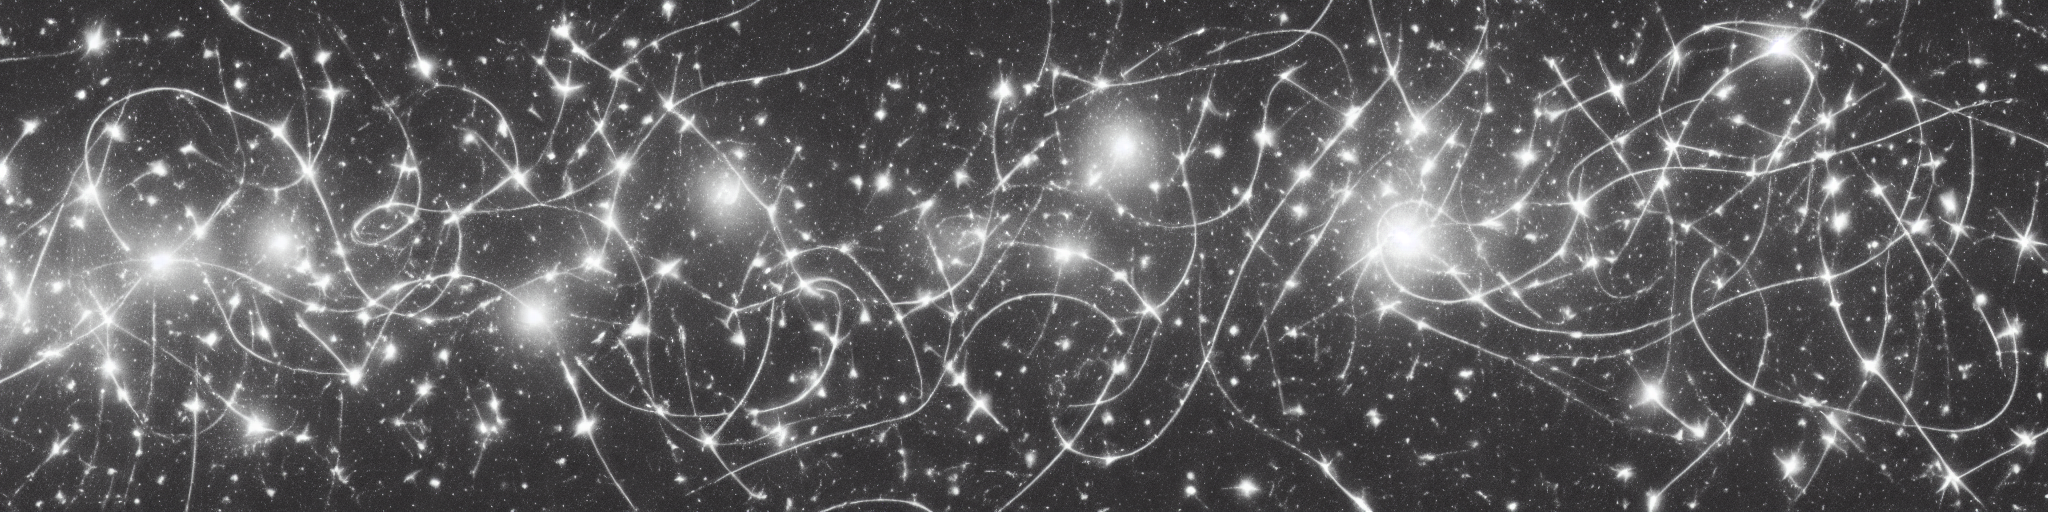
\includegraphics[width=1.18\paperwidth]{header2.png}%
% \transparent{0.16}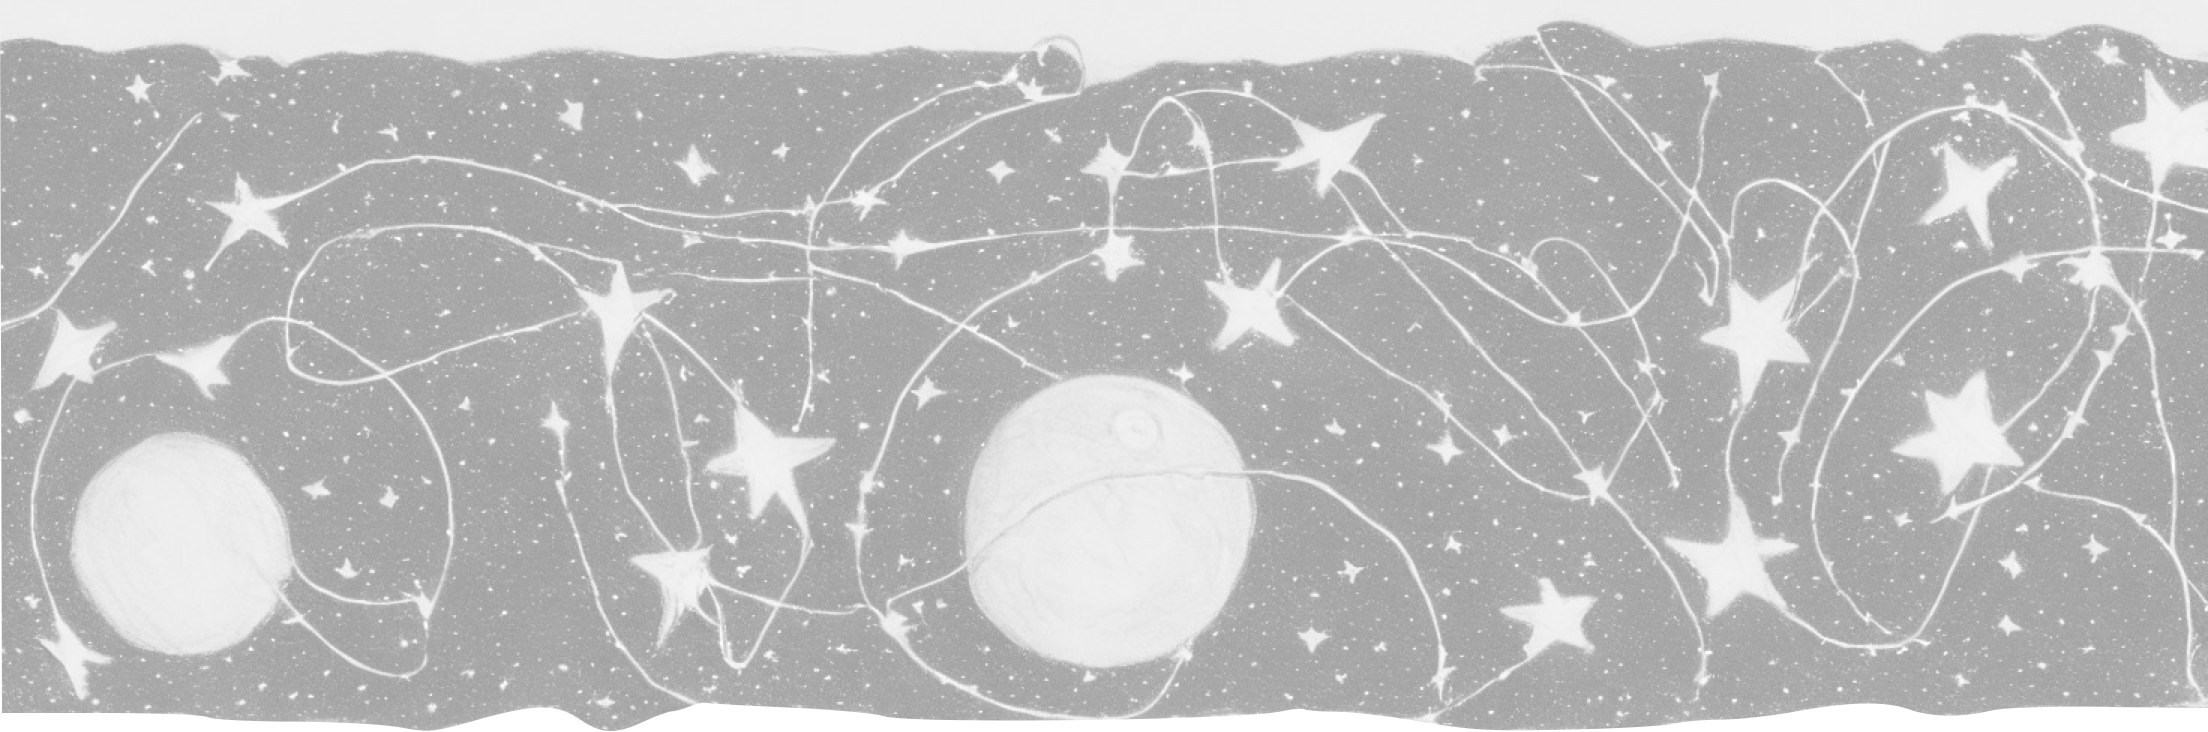
\includegraphics[width=1.04\paperwidth]{header.png}%
\vfill
}}}

\AddToShipoutPicture*{\BackgroundPic}

%%%%%%%%%%%%
% PDF setup

\ifpdf
  \usepackage[pdftex]{hyperref}
\else
  \usepackage[hypertex]{hyperref}
\fi
\hypersetup{
    letterpaper,
    colorlinks,
    linkcolor=linkcolor!\myshade!black,
    urlcolor=linkcolor!\myshade!black,
    pdfpagemode=none,
    pdftitle={Siddharth Mishra-Sharma's CV},
    pdfauthor={Siddharth Mishra-Sharma},
    pdfsubject={Siddharth Mishra-Sharma's CV},
    pdfkeywords={}
}

%%%%%%%%%%%%
% Toggle for printing phone number

% Get environmental variable ENV
\newcommand{\getenv}[2][]{%
  \CatchFileEdef{\temp}{"|kpsewhich --var-value #2"}{\endlinechar=-1}%
  \if\relax\detokenize{#1}\relax\temp\else\let#1\temp\fi}

\getenv[\ENV]{ENV}

% Print phone number ONLY if not compiling online GitHub version
\ifthenelse{\equal{\ENV}{GIT}}
  {
   \newcommand{\phone}{}%
  }
  {
   \newcommand{\phone}{\faMobile\hspace{1mm}\href{tel:16099330103}{+1 609-933-0103}}%
  }
%%%%%%%%%%%%

%%%%%%%%%%%%
% Margin setup
\oddsidemargin=-0.4in
\evensidemargin=-0.4in
\textwidth=7.2in
\headheight=-0.6in
\topmargin=0.12in
\textheight=9.6in
%%%%%%%%%%%%

%% Setup the header and footer
\pagestyle{fancy}
\fancyhf{}
\cfoot{Page\ \thepage\ of\ \pageref*{LastPage}}
\renewcommand{\headrulewidth}{0pt}
\renewcommand{\footrulewidth}{0.8pt}

\setlength{\tabcolsep}{0in}
\hyphenchar\font=-1

% Change bullet size
\makeatletter
\renewcommand\@biblabel[1]{\textbullet}
\makeatother

% Packed itemize environment
\newenvironment{packed_itemize}{
\begin{itemize}[label=\raisebox{0.25ex}{\tiny$\bullet$}]
  \setlength{\itemsep}{3.7pt}
  \setlength{\parskip}{0pt}
  \setlength{\parsep}{0pt}}{\end{itemize}
}

% Packed enumerate environment
\newenvironment{packed_enumerate}[1][]{
\begin{etaremune}[#1]
  \setlength{\itemsep}{3.7pt}
  \setlength{\parskip}{0pt}
  \setlength{\parsep}{0pt}}{\end{etaremune}
}
 \fancypagestyle{style1}{
 \fancyhf{}
 \fancyhead[C]{style 1 with thin line}
 \fancyfoot[C]{\thepage}
 \renewcommand{\headrulewidth}{0.4pt}
 }

% \fancypagestyle{style2}{
% \fancyhf{}
% \fancyhead[C]{STYLE 2 WITH THICK LINE}
% \fancyfoot[C]{= \thepage{} =}
% \renewcommand{\headrulewidth}{1pt}
% }

\newcommand{\SubItem}[1]{
    {\setlength\itemindent{15pt} \item[-] #1}
}

\begin{document}

%%%%%%%%%%%%
%% Heading

\begin{center}
\begin{tabular*}{\textwidth}{@{\extracolsep{\fill}}lcr}
&\huge{\textbf{\sc{Siddharth Mishra-Sharma}}}&   \\
& 77 Massachusetts Ave, 26-648, 
Cambridge, MA 02139, USA &\\

&\faEnvelopeO\hspace{1mm}\href{mailto:smsharma@mit.edu}{\texttt{smsharma@mit.edu}} 
~~\phone
~~\faGlobe\hspace{1mm}\href{https://smsharma.io}{\texttt{smsharma.io}} 
~~\faGithub\hspace{1mm}\href{https://github.com/smsharma}{\texttt{github.com/smsharma}} 
% ~\faGithub\hspace{1mm}\href{https://github.com/smsharma}{\texttt{github.com/smsharma}} &
\vspace{0.5mm}
\\ 

\hline\hline

\end{tabular*}
\end{center}

\vspace{2.0mm}

%%%%%%%%%%%%

%%%%%%%%%%%%
%% Appointments 

\noindent
\begin{tabular*}{\textwidth}{l@{\extracolsep{\fill}}}
\large {\sc \Large{Academic Appointments}}\\
\hline
\end{tabular*}

% MIT
\noindent 
\\
\begin{tabular*}{\textwidth}{l@{\extracolsep{\fill}}r}
\textbf{Massachusetts Institute of Technology}, \small{Center for Theoretical Physics}  & \textbf {Cambridge, MA, USA}\\
\textbf{Harvard University}, \small{Department of Physics} & \textbf {Cambridge, MA, USA}\\
{NSF AI Institute for Artificial Intelligence and Fundamental Interactions}\\
\emph{IAIFI Fellow}  & {Sep. 2021 -- Present}  \vspace{2mm}\\
\end{tabular*}

% NYU
\noindent 
\\
\begin{tabular*}{\textwidth}{l@{\extracolsep{\fill}}r}
\textbf{New York University} & \textbf {New York, NY, USA}\\
{Center for Cosmology and Particle Physics}\\
\emph{Postdoctoral Associate}  & {Sep. 2018 -- Aug. 2021} \\  
\end{tabular*}
\vspace{2.0mm}

%%%%%%%%%%%%
%% Education 

\noindent
\begin{tabular*}{\textwidth}{l@{\extracolsep{\fill}}}
\large {\sc \Large{Education}}\\
\hline
\end{tabular*}

% Princeton
\noindent 
\\
\begin{tabular*}{\textwidth}{l@{\extracolsep{\fill}}r}
\textbf{Princeton University}  & \textbf {Princeton, NJ, USA}\vspace{0mm}\\
{Ph.D. in Physics}  & {Sep. 2013 -- Aug. 2018} \vspace{.0mm} \\  
{Advisor: Mariangela Lisanti}& {} \vspace{.0mm} \\
{Thesis: \href{https://dataspace.princeton.edu/jspui/handle/88435/dsp012v23vx15d}{\emph{Extragalactic Searches for Dark Matter Annihilation}}}& {} \vspace{2mm} \\
% \small{M.A. awarded in Jan. 2015}& {} \vspace{2mm} \\

\end{tabular*}

% Cambridge
\noindent 
\\
\begin{tabular*}{\textwidth}{l@{\extracolsep{\fill}}r}
\textbf{University of Cambridge}  & \textbf {Cambridge, UK}\vspace{0mm}\\
{Part III of the Mathematical Tripos (M.Math.)} & {Oct. 2012 -- Jun. 2013}\vspace{0.0mm}\\ 
% \small{\emph{Specializing in Theoretical Physics}}\vspace{1mm}\\
{B.A. (Hons.) in Natural Sciences (Physical)} & {Oct. 2009 -- Jun. 2012} \\
% \small{\emph{Specializing in Physics}}\vspace{1mm}\\
\end{tabular*}
%\small{M.A. (Cantab) awarded in May 2016. \small{\emph{Note that this is an academic rank that may be given six years after the end of a first term at the University of Cambridge, and is not a postgraduate qualification.}}}\vspace{0mm}\\
\vspace{2.0mm}
%%%%%%%%%%%%

%%%%%%%%%%%%
%% Publications 

\noindent
\begin{tabular*}{\textwidth}{l@{\extracolsep{\fill}}}
\large {\sc \Large{Publications}}\\
\hline
\end{tabular*}\vspace{3.5mm}

\noindent
Primary contributions \emph{(Note: except where indicated with an asterisk\,$^*$, authors are listed in alphabetical order as per the standard in particle physics)}:

\begin{packed_enumerate}[start=34]

  \item L. Heinrich, \underline{S. Mishra-Sharma}, C. Pollard, P. Windischhofer, \emph{Hierarchical Neural Simulation-Based Inference Over Event Ensembles} \href{https://arxiv.org/abs/2306.12584}{[arXiv:2306.12584]}
  
  \item $^*$G. Zhang, \underline{S. Mishra-Sharma}, C. Dvorkin, \emph{Inferring subhalo effective density slopes from strong lensing observations with neural likelihood-ratio estimation}, \href{https://doi.org/10.1093/mnras/stac3014}{Mon.Not.Roy.Astron.Soc. 517 (2022) 4317} \href{https://arxiv.org/abs/2208.13796}{[arXiv:2208.13796]}

  \item $^*$T. Nguyen, \underline{S. Mishra-Sharma}, L. Necib, \emph{Uncovering dark matter density profiles in dwarf galaxies with graph neural networks}
  \begin{packed_itemize}
      \item {\href{https://journals.aps.org/prd/abstract/10.1103/PhysRevD.107.043015}{Phys.Rev. \textbf{D107} (2022) 043015}} \href{https://arxiv.org/abs/2208.12825}{[arXiv:2208.12825]}
      \item Machine Learning for Astrophysics Workshop at the Thirty-ninth International Conference on Machine Learning (ICML 2022) \href{https://ml4astro.github.io/icml2022/}{[Spotlight Oral]} \href{https://ml4astro.github.io/icml2022/assets/38.pdf}{[Paper]}
    \end{packed_itemize}
    
  \item $^*$\underline{S. Mishra-Sharma}, G. Yang, \emph{Strong Lensing Source Reconstruction Using Continuous Neural Fields}, {Machine Learning for Astrophysics Workshop at the Thirty-ninth International Conference on Machine Learning (ICML 2022)} \href{https://ml4astro.github.io/icml2022/}{[Spotlight Oral]} \href{https://arxiv.org/abs/2206.14820}{[arXiv:2206.14820]}
   
  % \item $^*$T. Nguyen, \underline{S. Mishra-Sharma} and L. Necib, \emph{Uncovering dark matter density profiles in dwarf galaxies with graph neural networks}, {Machine Learning for Astrophysics Workshop at the Thirty-ninth International Conference on Machine Learning (ICML 2022)} [Spotlight Oral] \href{https://ml4astro.github.io/icml2022/assets/38.pdf}{[Paper]}

  \item A. Caputo, H. Liu, \underline{S. Mishra-Sharma}, M. Pospelov, J.T. Ruderman, \emph{A Stimulating Explanation of the Extragalactic Radio Background}, \href{https://journals.aps.org/prd/abstract/10.1103/PhysRevD.107.123033}{Phys.Rev. \textbf{D107} (2023) 123033} \href{https://arxiv.org/abs/2206.07713}{[arXiv:2206.07713]}

  \item  $^*$\underline{S. Mishra-Sharma}, K. Cranmer, \emph{A neural simulation-based inference approach for characterizing the Galactic Center $\gamma$-ray excess}
    \begin{packed_itemize}
      \item {\href{https://journals.aps.org/prd/abstract/10.1103/PhysRevD.105.063017}{Phys.Rev. \textbf{D105} (2022) 063017} \href{https://arxiv.org/abs/2110.2110.06931}{[arXiv:2110.2110.06931]}}
      \item {Machine Learning and the Physical Sciences Workshop at the 35th Conference on Neural Information Processing Systems (NeurIPS 2021) \href{https://ml4physicalsciences.github.io/2020/files/NeurIPS_ML4PS_2020_20.pdf}{[Paper]}\,\href{https://ml4physicalsciences.github.io/2020/files/NeurIPS_ML4PS_2020_20_poster.pdf}{[Poster]}}
    \end{packed_itemize}

%  \item  $^*$\underline{S. Mishra-Sharma} and K. Cranmer, \emph{Characterizing $\gamma$-ray maps of the Galactic Center with neural density estimation}, Machine Learning and the Physical Sciences Workshop at the 35th Conference on Neural Information Processing Systems (NeurIPS 2021) \href{https://ml4physicalsciences.github.io/2020/files/NeurIPS_ML4PS_2020_20.pdf}{[Paper]}\,\href{https://ml4physicalsciences.github.io/2020/files/NeurIPS_ML4PS_2020_20_poster.pdf}{[Poster]}

  \item \underline{S. Mishra-Sharma}, \emph{Inferring dark matter substructure with astrometric lensing beyond the power spectrum}  
  \begin{packed_itemize}
    \item {\href{https://doi.org/10.1088/2632-2153/ac494a}{Mach.Learn.Sci.Tech. \textbf{3} (2022) 01LT03} \,\href{https://arxiv.org/abs/2110.01620}{[arXiv:2110.01620]}}
    \item {{Machine Learning and the Physical Sciences Workshop at the 35th Conference on Neural Information Processing Systems (NeurIPS 2021)} \href{https://ml4physicalsciences.github.io/2021/files/NeurIPS_ML4PS_2021_22_poster.png}{[Poster]}}
    \end{packed_itemize}

  \item $^*$\underline{S. Mishra-Sharma}, K. Cranmer, \emph{Semi-parametric $\gamma$-ray modeling with Gaussian processes and variational inference}, {Machine Learning and the Physical Sciences Workshop at the 34rd Conference on Neural Information Processing Systems (NeurIPS 2020)} \href{https://ml4physicalsciences.github.io/2020/files/NeurIPS_ML4PS_2020_20.pdf}{[Paper]}\,\href{https://ml4physicalsciences.github.io/2020/files/NeurIPS_ML4PS_2020_20_poster.pdf}{[Poster]}\,\href{https://arxiv.org/abs/2010.10450}{[arXiv:2010.10450]} 

  \item A. Caputo, H. Liu, \underline{S. Mishra-Sharma}, M. Pospelov, J.T. Ruderman, A. Urbano, \emph{Edges and Endpoints in 21-cm Observations from Resonant Photon Production},  \href{https://journals.aps.org/prl/abstract/10.1103/PhysRevLett.127.011102}{Phys.Rev.Lett. \textbf{127} (2021) 011102}   \href{https://arxiv.org/abs/2009.03899}{[arXiv:2009.03899]}

  \item $^*$J.J. Somalwar, L.J. Chang, \underline{S. Mishra-Sharma}, M. Lisanti, \emph{Harnessing the Population Statistics of Subhalos to Search for Annihilating Dark Matter}, \href{https://iopscience.iop.org/article/10.3847/1538-4357/abc87d}{Astrophys.J. \textbf{906} (2021) no.1, 57} \href{https://arxiv.org/abs/2009.00021}{[arXiv:2009.00021]}

  \item A. Caputo, H. Liu, \underline{S. Mishra-Sharma}, J.T. Ruderman, \emph{Modeling Dark Photon Oscillations in Our Inhomogeneous Universe}, \href{https://journals.aps.org/prd/abstract/10.1103/PhysRevD.102.103533}{Phys.Rev. \textbf{D102} (2020) 103533}   \href{https://arxiv.org/abs/2004.06733}{[arXiv:2004.06733]}

  \item \underline{S. Mishra-Sharma}, K. Van Tilburg, N. Weiner, \emph{Power of Halometry}, \href{https://journals.aps.org/prd/abstract/10.1103/PhysRevD.102.023026}{Phys.Rev. \textbf{D102} (2020) 023026} [Editors' Suggestion and Featured in \emph{Physics}; \href{https://physics.aps.org/articles/v13/s98}{Synopsis}]  \href{https://arxiv.org/abs/2003.02264}{[arXiv:2003.02264]}

  \item $^*$M. Buschmann, N.L. Rodd, B.R. Safdi, L.J. Chang, \underline{S. Mishra-Sharma}, M. Lisanti, O. Macias \emph{Foreground Mismodeling and the Point Source Explanation of the Fermi Galactic Center Excess},  \href{https://journals.aps.org/prd/abstract/10.1103/PhysRevD.102.023023}{Phys.Rev. \textbf{D102} (2020) 023023} \href{https://arxiv.org/abs/2002.12373}{[arXiv:2002.12373]} 

  \item A. Caputo, H. Liu, \underline{S. Mishra-Sharma}, J.T. Ruderman, \emph{Dark Photon Oscillations in Our Inhomogeneous Universe}, \href{https://journals.aps.org/prl/abstract/10.1103/PhysRevLett.125.221303}{Phys.Rev.Lett. \textbf{125} (2020) 221303}  \href{https://arxiv.org/abs/2002.05165}{[arXiv:2002.05165]}

  \item $^*$J. Brehmer, K. Cranmer, \underline{S. Mishra-Sharma}, F. Kling, G. Louppe, \emph{Mining gold: Improving simulation-based inference with latent information}, {Machine Learning and the Physical Sciences Workshop at the 33rd Conference on Neural Information Processing Systems (NeurIPS 2019)} \href{https://ml4physicalsciences.github.io/files/NeurIPS_ML4PS_2019_16.pdf}{[Paper]}

  \item $^{*\dagger}$J. Brehmer, $^\dagger$\underline{S. Mishra-Sharma}, J. Hermans, G. Louppe, K. Cranmer, \emph{Mining for Dark Matter Substructure: Inferring subhalo population properties from strong lenses with machine learning}, \href{https://iopscience.iop.org/article/10.3847/1538-4357/ab4c41}{Astrophys.J. \textbf{886} (2019) no.1, 49} \href{https://arxiv.org/abs/1909.02005}{[arXiv:1909.02005]} ($^\dagger$\emph{Equal contribution})

  \item $^*$L.J. Chang, \underline{S. Mishra-Sharma}, M. Lisanti, M. Buschmann, N.L. Rodd, B.R. Safdi, \emph{Characterizing the Nature of the Unresolved Point Sources in the Galactic Center: An Assessment of Systematic Uncertainties},  \href{https://journals.aps.org/prd/abstract/10.1103/PhysRevD.101.023014}{Phys.Rev. \textbf{D101} (2020) 023014} \href{https://arxiv.org/abs/1908.10874}{[arXiv:1908.10874]}, 

  \item L.J. Chang, M. Lisanti, \underline{S. Mishra-Sharma}, \emph{Search for Dark Matter Annihilation in the Milky Way Halo}, \href{https://journals.aps.org/prd/abstract/10.1103/PhysRevD.98.123004}{Phys.Rev. \textbf{D98} (2018) 123004} \href{https://arxiv.org/abs/1804.04132}{[arXiv:1804.04132]}

  \item $^*$\underline{S. Mishra-Sharma}, D. Alonso, J. Dunkley, \emph{Neutrino masses and beyond-$\Lambda$CDM cosmology with LSST and future CMB experiments}, \href{https://journals.aps.org/prd/abstract/10.1103/PhysRevD.97.123544}{Phys.Rev. \textbf{D97} (2018) 123544}  \href{https://arxiv.org/abs/1803.07561}{[arXiv:1803.07561]}

  \item R. Bartels, D. Hooper, T. Linden, \underline{S. Mishra-Sharma}, N.L. Rodd, B.R. Safdi, T.R. Slatyer, \emph{Comment on ``Characterizing the population of pulsars in the Galactic bulge with the
  {\it Fermi} Large Area Telescope'' [arXiv:1705.00009\MakeLowercase{v}1]}, \href{https://www.sciencedirect.com/science/article/pii/S2212686418300268}{Phys.Dark Univ. \textbf{20} (2018) 88-94} \href{https://arxiv.org/abs/1710.10266}{[arXiv:1710.10266]}

  \item M. Lisanti, \underline{S. Mishra-Sharma}, N.L. Rodd, B.R. Safdi, \emph{Mapping Extragalactic Dark Matter Annihilation with Galaxy Surveys: A Systematic Study of Stacked Group Searches},  \href{https://journals.aps.org/prd/abstract/10.1103/PhysRevD.97.063005}{Phys.Rev. \textbf{D97} (2018) 063005} \href{https://arxiv.org/abs/1709.00416}{[arXiv:1709.00416]}

  \item M. Lisanti, \underline{S. Mishra-Sharma}, N.L. Rodd, B.R. Safdi, \emph{Search for Dark Matter Annihilation in Galaxy Groups},  \href{https://journals.aps.org/prl/abstract/10.1103/PhysRevLett.120.101101}{Phys.Rev.Lett. \textbf{120} (2018) 101101} \href{https://arxiv.org/abs/1708.09385}{[arXiv:1708.09385]}

  \item T. Cohen, M. Lisanti, H. K. Lou, \underline{S. Mishra-Sharma}, \emph{LHC Searches for Dark Sector Showers},  \href{https://link.springer.com/article/10.1007/JHEP11(2017)196}{JHEP \textbf{11}, 196 (2017)}  \href{https://arxiv.org/abs/1707.05326}{ [arXiv:1707.05326]}

  \item \underline{S. Mishra-Sharma}, N.L. Rodd, B.R. Safdi, \emph{NPTFit: A code package for Non-Poissonian Template Fitting},  \href{http://iopscience.iop.org/article/10.3847/1538-3881/aa6d5f/meta}{Astron.J. \textbf{153} (2017) no.6, 253}  \href{https://arxiv.org/abs/1612.03173}{ [arXiv:1612.03173]}

  \item Y. Kahn, G. Krnjaic, \underline{S. Mishra-Sharma}, T.M.P. Tait, \emph{Light Weakly Coupled Axial Forces: Models, Constraints, and Projections},  \href{https://link.springer.com/article/10.1007%2FJHEP05%282017%29002}{JHEP \textbf{05}, 002 (2017)}  \href{https://arxiv.org/abs/1609.09072}{[arXiv:1609.09072]}

  \item M. Lisanti, \underline{S. Mishra-Sharma}, L. Necib, B.R. Safdi, \emph{Deciphering Contributions to the Extragalactic Gamma-Ray Background from 2 GeV to 2 TeV},  \href{http://iopscience.iop.org/article/10.3847/0004-637X/832/2/117/meta}{Astrophys.J. \textbf{832} (2016) no.2, 117} \href{https://arxiv.org/abs/1606.04101}{[arXiv:1606.04101]}

  \item S.K. Lee, M. Lisanti, \underline{S. Mishra-Sharma}, B.R. Safdi, \emph{Modulation Effects in Dark Matter-Electron Scattering Experiments}, \href{https://journals.aps.org/prd/abstract/10.1103/PhysRevD.92.083517}{Phys.Rev. \textbf{D92} (2015) 083517} \href{https://arxiv.org/abs/1508.07361}{[arXiv:1508.07361]}
\end{packed_enumerate}

\noindent
Contributions to white papers and as part of larger collaborations:

\begin{packed_enumerate}[start=7]

  \item C. Dvorkin, \underline{S. Mishra-Sharma} \emph{et al.}, \emph{Machine Learning and Cosmology: Snowmass 2021 White Paper} \href{https://arxiv.org/abs/2203.08056}{[arXiv:2203.08056]}

  \item K. Boddy \emph{et al.} (including \underline{S. Mishra-Sharma}), \emph{Snowmass2021 theory frontier white paper: Astrophysical and cosmological probes of dark matter},  \href{https://www.sciencedirect.com/science/article/pii/S2214404822000349}{J.HEAp 35 (2022) 112-138}  \href{https://arxiv.org/abs/2203.08056}{[arXiv:2203.08056]}

  \item R. Leane \emph{et al.} (including \underline{S. Mishra-Sharma}), \emph{Snowmass2021 Cosmic Frontier White Paper: Puzzling Excesses in Dark Matter Searches and How to Resolve Them} \href{https://arxiv.org/abs/2203.06859}{[arXiv:2203.06859]}

  \item J. Alimena \emph{et al.} (including \underline{S. Mishra-Sharma}), \emph{Searching for long-lived particles beyond the Standard Model at the Large Hadron Collider}, \href{https://iopscience.iop.org/article/10.1088/1361-6471/ab4574}{J.Phys.G 47 (2020) 090501} \href{https://arxiv.org/abs/1903.04497}{[arXiv:1903.04497]}

  \item S. Algeri \emph{et al.} (including \underline{S. Mishra-Sharma}), \emph{Statistical challenges in the search for dark matter} \href{https://arxiv.org/abs/1807.09273}{[arXiv:1807.09273]}

  \item DarkSide Collaboration (including \underline{S. Mishra-Sharma}), \emph{Constraints on Sub-GeV Dark Matter-Electron Scattering from the DarkSide-50 Experiment}, \href{https://journals.aps.org/prl/abstract/10.1103/PhysRevLett.121.111303}{Phys.Rev.Lett. \textbf{121} (2018) 111303} \href{https://arxiv.org/abs/1802.06998}{[arXiv:1802.06998]}

  \item DarkSide Collaboration (including \underline{S. Mishra-Sharma}), \emph{Low-Mass Dark Matter Search with the DarkSide-50 Experiment}, \href{https://journals.aps.org/prl/abstract/10.1103/PhysRevLett.121.081307}{Phys.Rev.Lett. \textbf{121} (2018) 081307}  \href{https://arxiv.org/abs/1802.06994}{[arXiv:1802.06994]}
\end{packed_enumerate}
\vspace{2.0mm}

% \newpage

%%%%%%%%%%%%

%%%%%%%%%%%%
%% Talks 

\noindent
\begin{tabular*}{\textwidth}{l@{\extracolsep{\fill}}}
\large {\sc \Large{Seminars, Colloquia, and Conference Talks}}\\
\hline
\end{tabular*}\vspace{3.5mm}

\noindent
Invited talks:
\begin{packed_itemize}
  \item MIAPbP Workshop on Differentiable and Probabilistic Programming \hfill Munich, Germany, Jun. 2023
  \item Status of the Galactic Center Excess Workshop \hfill New Brunswick, NJ, Jun. 2023
  \item Simons Foundation MATH+X Symposium \hfill Hella, Iceland, May. 2023
  \item Cosmic Connections: ML X Astrophysics (Flatiron Institute) \hfill New York, NY, May. 2023
  \item Harvard Center for Astrophysics ITC Lunch Talk  \hfill Cambridge, MA, Apr. 2023
  \item Aspen Center for Physics Winter Session \hfill Aspen, CO, Mar. 2023
  \item Normal Computing (Probabilistic AI Startup; Remote) \hfill Feb. 2023
  \item Yale Astronomy Colloquium \hfill New Haven, CT, Feb. 2023
  \item Mila ML for the Physical Sciences Reading Group \hfill Montr\'eal, Quebec, Jan. 2023
  \item McGill Space Institute Astronomy Seminar \hfill Montr\'eal, Quebec, Jan. 2023
  \item Nature of Dark Matter on Small Scales Meeting (Remote) \hfill  Oct. 2022
  \item Dagstuhl Seminar: Bridging Data-driven and Mechanistic Modelling \hfill Dagstuhl, Germany, Sep. 2022
  \item Hammers \& Nails Workshop 2022 \hfill Rehovot, Israel, Aug. 2022
  \item ICML 2022 ML4Astro Workshop (Spotlight oral) \hfill Baltimore, MD, May. 2022
  \item Physics $\cap$ ML Seminar (Remote at \href{http://www.physicsmeetsml.org//}{\texttt{physicsmeetsml.org}}) \hfill May. 2022
  \item Harvard CHASC Astrostatistics Seminar (Remote)  \hfill Apr. 2022
  \item University of Illinois Urbana-Champaign Phenomenology Seminar  \hfill Urbana, IL, Mar. 2022
  \item Harvard High Energy Theory Seminar \hfill Cambridge, MA, Mar. 2022
  \item American Astronomical Society 239th Meeting (Invited panel)  \hfill Salt Lake City, UT, Jan. 2022
  \item Harvard LPPC (High Energy Experiment) Seminar \hfill Cambridge, MA, Nov. 2021
  \item Rutgers High Energy Theory Seminar \hfill New Brunswick, NJ, Oct. 2021
  \item Instituto de Astrof\'{i}sica de Canarias Astrophysics Seminar (Remote) \hfill Sep. 2021
  \item Stony Brook University YITP Seminar (Remote) \hfill Mar. 2021
  \item SLAC AI Seminar Series (Remote) \hfill Feb. 2021
  \item Northeastern University Physics Colloquium (Remote) \hfill Feb. 2021
  \item Carnegie Observatories ``Lunch Talk'' Seminar (Remote) \hfill Feb. 2021
  \item BSM PANDEMIC Seminar  (Remote at \href{https://www.bsmpandemic.com/}{\texttt{bsmpandemic.com}}) \hfill Nov. 2020
  \item SLAC Elementary Particle Physics Seminar (Remote) \hfill Jul. 2020
  \item University of Amsterdam GRAPPA Colloquium (Remote) \hfill May 2020
  \item Princeton Pheno \& Vino Seminar (Remote) \hfill Apr. 2020
  \item CERN-TH BSM Forum (Remote) \hfill  Apr. 2020
  \item Machine Learning for Astrophysicists Seminar (Remote at \href{https://docs.google.com/document/d/1GGtE-YIuAWlmpKSr38_kyiF-Fklszhkh4FkiYWzBAho/pub}{\texttt{mlclub.net}}) \hfill  Mar. 2020
  \item University of Michigan LCTP Brown Bag Seminar \hfill Ann Arbor, MI, Jan. 2020
  \item Stony Brook University Particle Physics Seminar \hfill Stony Brook, NY, Nov. 2019
  \item Minnesota High Energy Theory Lunchtime Seminar \hfill  Minneapolis, MN, Nov. 2019
  \item Brown Astrophysics Seminar Series \hfill Providence, RI, May 2019
  \item Particles, Strings and Cosmology (PASCOS) 2018 \hfill Cleveland, OH, Jun. 2018
  \item Recontres de Blois 2018 \hfill Blois, France, Jun. 2018
  \item Princeton Astrophysics/IAS Cosmology Lunch Seminar \hfill Princeton, NJ, May 2018
  \item Fermilab Particle Astrophysics Seminar \hfill Batavia, IL, Mar. 2018
  \item Workshop on Statistical Challenges in the Search for Dark Matter \hfill Banff, Canada, Feb. 2018
  \item Maryland Elementary Particle Theory Seminar \hfill College Park, MD, Nov. 2017
  \item Rutgers High Energy Theory Seminar \hfill New Brunswick, NJ, Nov. 2017
  \item Cornell Particle Theory Seminar \hfill Ithaca, NY, Nov. 2017
  \item Caltech Particle Theory Seminar \hfill Pasadena, CA, Oct. 2017
  \item UC Irvine Joint Particle Seminar \hfill Irvine, CA, Oct. 2017
  \item ICTP LHC Long-Lived Particles Community Workshop (Remote) \hfill Oct. 2017
  \item Oxford Dalitz Seminar in Fundamental Physics  \hfill Oxford, UK, Oct. 2017
  \item KIPAC Tea Talk  \hfill Stanford, CA, Sep. 2017
  \item UC Santa Cruz Institute for Particle Physics Seminar  \hfill Santa Cruz, CA, Sep. 2017
  \item Berkeley 4D Seminar  \hfill Berkeley, CA, Sep. 2017
  \item MIT BSM Journal Club \hfill Boston, MA, Nov. 2016
\end{packed_itemize}

\noindent
Internal talks:
\begin{packed_itemize}
  \item IAIFI Seminar \hfill Cambridge, MA, Apr. 2022
  \item MIT CTP Nuclear and Particle Theory Seminar \hfill Cambridge, MA, Feb. 2022
  \item MIT CTP Graduate Student Lunch Seminar (Remote) \hfill Mar. 2021
  \item MIT QCD-DM-BSM-LHC Journal Club (Remote) \hfill Mar. 2021
  \item NYU CCPP Brown Bag Seminar \hfill New York, NY, Apr. 2019
  \item Princeton Pheno \& Vino Seminar \hfill Princeton, NJ, Apr. 2017
\end{packed_itemize}
%\newpage

\noindent
Contributed talks:
\begin{packed_itemize}
  \item MIT Statistics and Data Science Conference  \hfill Cambridge, MA, Apr. 2022
  \item WFIRST Science Meeting (Flatiron Institute) \hfill New York, NY, Mar. 2020
  \item LSST Dark Matter Workshop \hfill Chicago, IL, Aug. 2019
  \item SUSY 2019 \hfill Corpus Christi, TX, May 2019
  \item Phenomenology Symposium (Pheno) 2019 \hfill Pittsburgh, PA, May 2019
  \item Dark Matter, Neutrinos and their Connection (DA$\nu$CO) \hfill Odense, Denmark, Aug. 2017
  \item TeV Particle Astrophysics (TeVPA) 2017 \hfill Columbus, OH, Aug. 2017 
  \item Phenomenology Symposium (Pheno) 2017 \hfill Pittsburgh, PA, May 2017 
  \item APS April Meeting 2017 \hfill Washington, DC, Jan. 2017 
  \item TeV Particle Astrophysics (TeVPA) 2016 \hfill Geneva, Switzerland, Sep. 2016 
  \item Gamma Rays and Dark Matter Workshop \hfill Obergurgl, Austria, Dec. 2015
  \item Phenomenology Symposium (Pheno) 2015 \hfill Pittsburgh, PA, May 2015
\end{packed_itemize}
\vspace{2.0mm}

%%%%%%%%%%%%

%%%%%%%%%%%%
%% Prizes and Honours 

\noindent
\begin{tabular*}{\textwidth}{l@{\extracolsep{\fill}}}
\large {\sc \Large{Awards}}\\
\hline
\end{tabular*}\vspace{1.mm}

\begin{packed_itemize}
  \item IAIFI Fellowship, \emph{NSF AI Institute for Artificial Intelligence and Fundamental Interactions} \hfill 2021 \\ \emph{Awarded towards independent postdoctoral research at the intersection of physics and \\ artificial intelligence}
  \item Department Teaching Award, \emph{Princeton Department of Physics}  \hfill 2018 \\ \emph{Awarded for excellence in the role of Assistant in Instruction for courses taught at Princeton}
  \item Kusaka Memorial Prize in Physics, \emph{Princeton Department of Physics} \hfill 2017 \\ \emph{Awarded to physics graduate students who have shown outstanding performance in research \\ and professional promise}
  \item Princeton Graduate School Impact Award, \emph{Princeton Graduate School} \hfill 2016 \\ \emph{Awarded to an individual in the community that has made a difference during their time \\ at Princeton}
  \item Princeton First-Year Graduate Fellowship, \emph{Princeton University} \hfill 2013 \\ \emph{Awarded towards the first year of graduate study at Princeton}
  \item Hugo de Balsham Prize, \emph{Peterhouse, University of Cambridge}  \hfill 2012 \\ \emph{Awarded for exceptional academic distinction at Peterhouse, Cambridge}
  \item Peter Scheuer Scholarship in Natural Sciences, \emph{Peterhouse, University of Cambridge} \hfill 2011, 2012 \\ \emph{Awarded for exceptional academic performance in the Cambridge second and third year \\ Tripos examinations}
  \item Senior Academic Scholarship, \emph{Peterhouse, University of Cambridge} \hfill 2010\\ \emph{Awarded for exceptional academic performance in the Cambridge first year Tripos examinations}
\end{packed_itemize}
\vspace{2.0mm}

%%%%%%%%%%%%

%%%%%%%%%%%%
%% Broader impact
 
\noindent
\begin{tabular*}{\textwidth}{l@{\extracolsep{\fill}}}
\large {\sc \Large{Broader Impact and Community}}\\
\hline
\end{tabular*}\vspace{1.mm}

\begin{packed_itemize}
  \item \emph{Organizer}, NeurIPS Machine Learning and the Physical Sciences Workshop \hfill 2022
  \item \emph{Journal Reviewer}, Astrophys. J., Phys.Rev.{D}, Phys.Rev.Lett., Comput.Phys.Commun., JHEP,  JCAP, Journal of Open Source Software, MLST
  \item \emph{Workshop Reviewer}, \scriptsize{NeurIPS Machine Learning and the Physical Sciences Workshop, NeurIPS AI for Science Workshop, ICLR Workshop on Deep Generative Models for Highly Structured Data, ICLR Workshop on Neural Fields, ICML Workshop on Machine Learning for Astrophysics, ICML Workshop on Structured Probabilistic Inference \& Generative Modeling, ICML Workshop on Synergy of Scientific and Machine Learning Modeling}\normalsize
  \item \emph{Grant Review Panel}, Department of Energy ASCR Leadership Computing Challenge \hfill 2023
  \item \emph{Grant Review Panel}, NASA ROSES/Astrophysics Research and Analysis \hfill 2023
  \item \emph{Chair}, IAIFI Speaker Selection Committee  \hfill 2023 -- Present
  \item \emph{Member}, IAIFI Computing Committee  \hfill 2022 -- Present
  \item \emph{Member}, IAIFI Early Career and Equity Committee  \hfill 2021 -- 2023
  \item \emph{Organizer}, NYU CCPP Particle Physics Seminar \hfill 2019 -- 2020
  % \item \emph{Member}, Princeton University Student Life Committee \hfill 2016 -- 2018
  % \item \emph{Member}, Princeton Graduate Housing Advisory Board \hfill 2016 -- 2018
  \item \emph{Vice Chair}, Princeton Graduate College House Committee \hfill 2016 -- 2018
  \item \emph{Subject Representative}, Princeton Graduate Student Government Assembly \hfill 2013 -- 2017
  \item \emph{Organizer}, Princeton Physics Department Open House Committee  \hfill 2015 -- 2016
  \item \emph{Chair}, Princeton Physics Graduate Student Council \hfill 2015 -- 2018
\end{packed_itemize}
\vspace{2.0mm}

%%%%%%%%%%%%

%%%%%%%%%%%%
%% Mentoring 

\noindent
\begin{tabular*}{\textwidth}{l@{\extracolsep{\fill}}}
\large {\sc \Large{Research Mentorship}}\\
\hline
\end{tabular*}\vspace{1.mm}

\begin{packed_itemize}
  \item Yitian Sun (Graduate, {MIT}) \hfill 2021 -- Present \\ \emph{Probabilistic programming and deep generative modeling for $\gamma$-ray data analysis}
  \item Aizhan Akhmetzhanova (Graduate, {Harvard}) \hfill 2021 -- Present \\ \emph{Simulation-based self-supervision for cosmological data compression and inference}
  \item Tri Nguyen (Graduate, {MIT}) \hfill 2021 -- Present \\ \emph{Inferring the shapes of dark matter halos with graph neural networks} \href{https://arxiv.org/abs/2208.12825}{[arXiv:2208.12825]}
  \item Gemma Zhang (Graduate, {Harvard}) \hfill 2021 -- 2022 \\ \emph{Inferring subhalo populations in strong lenses with likelihood-free inference} \href{https://arxiv.org/abs/2208.13796}{[arXiv:2208.13796]}
  \item Reuel Williams (Undergraduate, {Princeton})\hfill 2021 \\ \emph{Inferring the shapes of dark matter halos with graph neural networks} \href{https://arxiv.org/abs/2208.12825}{[arXiv:2208.12825]}
  \item Jean Somalwar (Undergraduate, {Princeton})\hfill 2019 -- 2020 \\ \emph{Searching for dark matter in Galactic subhalos using photon statistics} \href{https://arxiv.org/abs/2009.00021}{[arXiv:2009.00021]}
  \item Laura Chang (Graduate, {Princeton})\hfill 2018 -- 2020 \\ \emph{Searches for annihilating dark matter in the Milky Way} \href{https://arxiv.org/abs/1804.04132}{[arXiv:1804.04132]}\,\href{https://arxiv.org/abs/1908.10874}{[arXiv:1908.10874]}
  \end{packed_itemize}
\vspace{2.0mm}

%%%%%%%%%%%%

%%%%%%%%%%%%
%% Teaching 

\noindent
\begin{tabular*}{\textwidth}{l@{\extracolsep{\fill}}}
\large {\sc \Large{Teaching Experience}}\\
\hline
\end{tabular*}\vspace{3.5mm}

\noindent
Courses taught at MIT/IAIFI:
\begin{packed_itemize}
  \item IAIFI Summer School [Lectures on Generative Modeling] \hfill Summer 2023
  \item 8.16 Data Science in Physics \href{https://github.com/smsharma/sbi-lecture-mit}{[Guest Lecture]} \hfill Spring 2023
  \item IAIFI Summer School \href{https://github.com/smsharma/iaifi-summer-school-tutorials}{[Tutorials on Probabilistic Programming]} \hfill Summer 2022
  \item 8.S50 Computational Data Science in Physics \href{https://github.com/smsharma/prob-prog-8.S50-tutorial}{[Tutorials]} \hfill Winter 2022
\end{packed_itemize}

\noindent
Courses taught at Princeton:
\begin{packed_itemize}
  \item PHY235 Introduction to Research in Physics \hfill Spring 2018
  \item PHY312 Experimental Physics \hfill Spring 2018
  \item PHY115  Physics for Future Leaders \hfill Fall 2017
  \item PHY104  General Physics II \hfill Spring 2016
  \item PHY406 Nuclear and Elementary Particle Physics \hfill Fall 2015
  \item PHY106 Advanced Physics (Electromagnetism) \hfill Spring 2015
  \item MAT201 Calculus III (Multivariable Calculus) \hfill Fall 2014, 2015
  \item PHY105 Advanced Physics (Mechanics) \hfill Fall 2014
\end{packed_itemize}
\vspace{2.0mm}

%%%%%%%%%%%%

%%%%%%%%%%%%%
%%% Schools and Workshops
%
%\noindent
%\begin{tabular*}{\textwidth}{l@{\extracolsep{\fill}}}
%\large {\sc \Large{Workshops and Schools}}\\
%\hline
%\end{tabular*}\vspace{1.mm}
%
%\begin{packed_itemize}
%  \item \emph{Gaia} Sprint 2019 \hfill Santa Barbara, CA, Mar. 2019
%  \item Accelerating the Search for Dark Matter with Machine Learning \hfill Leiden, Netherlands, Jan. 2018
%  \item Prospects in Theoretical Physics (PiTP) \hfill Princeton, NJ, Jul. 2017
%  \item Theoretical Advanced Study Institute (TASI) \hfill Boulder, CO, Jun. 2016
%  \item Tri-Institute Summer School on Elementary Particles (TRISEP) \hfill Waterloo, Canada, Jul. 2015
%\end{packed_itemize}
%\vspace{2.0mm}
%
%%%%%%%%%%%%%

%%%%%%%%%%%%
%% Work Experience

\noindent
\begin{tabular*}{\textwidth}{l@{\extracolsep{\fill}}}
\large {\sc \Large{Research Training}}\\
\hline
\end{tabular*}\vspace{1.mm}

\begin{packed_itemize}
  \item CMS Experiment, CERN \hfill Geneva, Switzerland \\ \emph{Visiting Student Researcher} \hfill Aug. -- Sep. 2012 \\ \emph{Summer Student} \hfill Jun. -- Jul. 2011
  \item DAMTP, University of Cambridge \hfill Cambridge, UK \\ \emph{Summer Student} \hfill Jun. -- Jul. 2012
  \item Institute of Astronomy, University of Cambridge \hfill Cambridge, UK \\ \emph{Summer Student} \hfill Aug. -- Sep. 2011
  % \item CERN \hfill Geneva, Switzerland \\ \emph{Summer Student, CMS Experiment} \hfill Jun. -- Jul. 2011
\end{packed_itemize}
\vspace{2.0mm}

%%%%%%%%%%%%
%% References

\noindent
\begin{tabular*}{\textwidth}{l@{\extracolsep{\fill}}}
\large {\sc \Large{References}}\\
\hline
\end{tabular*}\vspace{1.mm}

\begin{packed_itemize}
  \item Mariangela Lisanti (Princeton University) \hfill \href{mailto:mlisanti@princeton.edu}{\texttt{mlisanti@princeton.edu}}
  \item Kyle Cranmer (University of Wisconsin, Madison) \hfill \href{mailto:kyle.cranmer@wisc.edu}{\texttt{kyle.cranmer@wisc.edu}}
  \item Tracy Slatyer (MIT) \hfill \href{mailto:tslatyer@mit.edu}{\texttt{tslatyer@mit.edu}}
  \item Jesse Thaler (MIT) \hfill \href{mailto:jthaler@mit.edu}{\texttt{jthaler@mit.edu}}
  \item Neal Weiner (New York University) \hfill \href{mailto:neal.weiner@nyu.edu}{\texttt{neal.weiner@nyu.edu}}
  \item Joshua Ruderman (New York University) \hfill \href{mailto:ruderman@nyu.edu}{\texttt{ruderman@nyu.edu}}
  \item Christoph Weniger (University of Amsterdam) \hfill \href{mailto:c.weniger@uva.nl}{\texttt{c.weniger@uva.nl}}
\end{packed_itemize}

%%%%%%%%%%%%

\vspace*{\fill}

\end{document}

% Jean, Laura, Reuel, 

